\lecture{Qualidade}{quality}

\lecturetitle{\course}{\insertlecture}

\frame{\maketitle}

\begin{frame}{\insertlecture}

\begin{itemize}[<+->]\setbeamercovered{transparent}
\item  Definição: Do latim \emph{qualitas}, qualidade é um atributo ou
  propriedade.

\item  Em negócios, engenharia e manufatura, qualidade tem o significado de
  não inferioridade ou superioridade sobre algum produto/serviço
  relacionado.

\item  Consumidores encaram qualidade do produto/serviço em termos das
  funções oferecidas e em comparação com concorrentes e com as
  próprias expectativas.

\item  Produtores percebem qualidade como o grau em que o produto é
  produzido corretamente.
\end{itemize}

\end{frame}

\frame{\author{}\date{}\title{\bf\Large (Alguns) Mestres da Qualidade}\maketitle}

\begin{frame}{Frederick Taylor (1856--1915)}
  
  \begin{columns}
    \begin{column}{.65\textwidth}
      Pai da administração científica, escreveu o livro "\emph{The Principles of Scientific Management}". Dentre seus estudos destacamos:
      \pause
      \begin{itemize}[<+->]\setbeamercovered{transparent}
      \item  Instruções sistemáticas e periódicas aos trabalhadores para melhoria da qualidade.
      \item Todo e qualquer trabalho necessita de um planejamento e metodologia prévios para atingir o máximo grau de eficiência.
      \item Supervisão funcional, onde todas as operações devem ser verificadas de acordo com as instruções programadas.
      \end{itemize}
    \end{column}
    \begin{column}{.35\textwidth}
      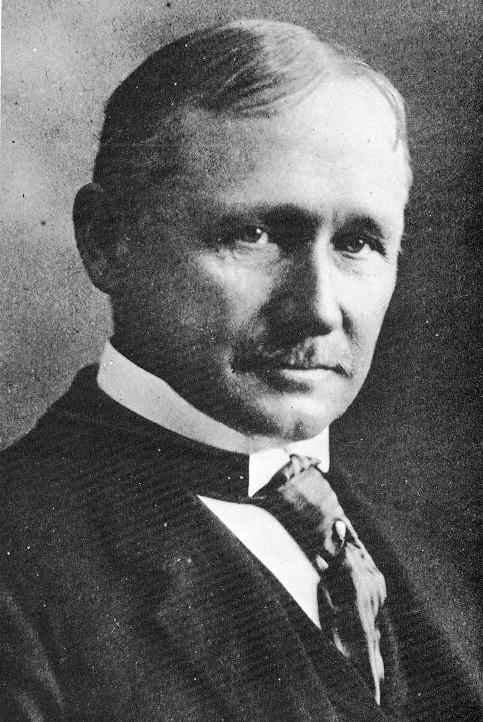
\includegraphics[scale=.3]{img/frederick-taylor.png}
    \end{column}
  \end{columns}

\end{frame}

\begin{frame}{William Edwards Deming (1900--1993)}
  
  \begin{columns}
    \begin{column}{.65\textwidth}
      Famoso por seus trabalhos na década de 1950, após a Segunda Guerra Mundial, principalmente do Japão. Segundo Deming, qualidade é um grau previsível de uniformidade, baixo custo e satisfação no mercado. Os pontos-chave de sua teoria são:
\begin{itemize}[<+->]\setbeamercovered{transparent}
\item Controle estatístico da qualidade.
\item Participação do trabalhador no processo de decisão.
\item Limitação das fontes de fornecimento, para que haja comprometimento do fornecedor com a qualidade da matéria-prima fornecida.
\end{itemize}
\end{column}
    \begin{column}{.35\textwidth}
      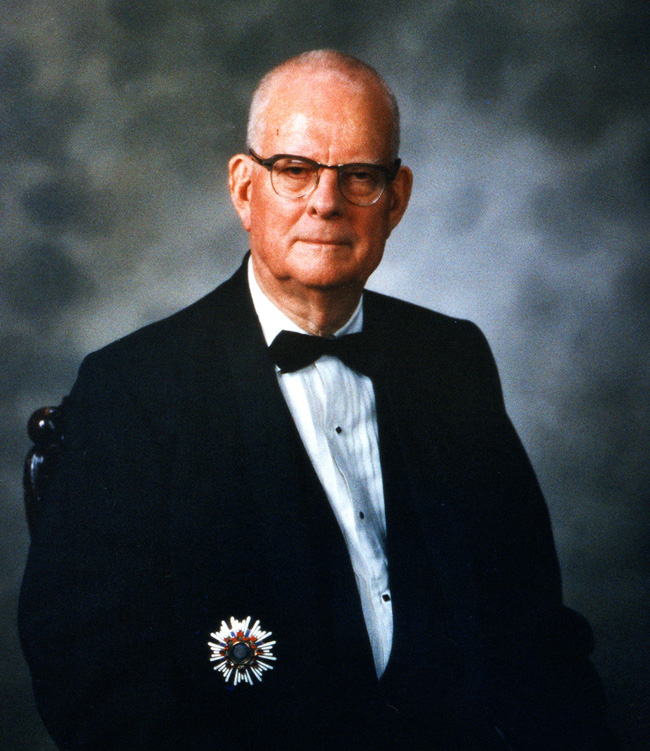
\includegraphics[scale=.175]{img/deming.png}
    \end{column}
  \end{columns}
\end{frame}

\begin{frame}{Armand Vallim Feigenbaum (1922--2014)}
  \small
  \begin{columns}
    \begin{column}{.65\textwidth}
      Foi um expert em qualidade da \emph{General Eletric} em Nova
      Iorque. Propôs o conceito de Gerenciamento da Qualidade Total,
      cujas principais diretrizes são:
      \pause
      \begin{enumerate}[<+->]\setbeamercovered{transparent}
      \item Qualidade de um produto está relacionado à percepção dos clientes e não da empresa (desenvolvedor).
      \item Qualidade e custo não estão separados.
      \item Qualidade exige comprometimento individual e da equipe.
      \item Qualidade e inovação estão relacionados.
      \item Qualidade não é temporária ou um conserto rápido é um contínuo processo de melhoria.
      \end{enumerate}
    \end{column}
    \begin{column}{.35\textwidth}
      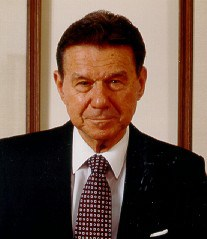
\includegraphics[scale=.4]{img/feigenbaum.png}
    \end{column}
  \end{columns}
\end{frame}

\begin{frame}{Joseph Moses Juran (1904--2008)}  
  \begin{columns}\scriptsize
    \begin{column}{.7\textwidth}
      Foi consultor de negócios famoso por seu trabalho com  gestão da qualidade. Criou o sistema de gestão JMS (\emph{Juram Management System}) que tem como essência:
      \pause
      \begin{description}[<+->]\setbeamercovered{transparent}
      \item[Planejamento da qualidade:] Identificação dos clientes e determinação de suas necessidades. Desenvolver um produto que atenda às necessidades.
      \item[Controle da qualidade:] Visa manter a produção dentro dos limites planejados para as diversas operações.
      \item[Melhoria da qualidade:] Identificação de pontos de melhoria, com posterior  aperfeiçoamento do processo de produção, equipe. Sugere o fornecimento de maior participação para a equipe em todos os níveis hierárquicos. Mantem-se contato constante com o cliente visando identificar possibilidades de aperfeiçoamento.
      \end{description}  
    \end{column}
      \begin{column}{.3\textwidth}
        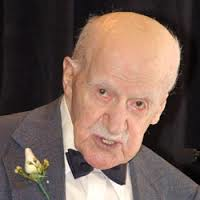
\includegraphics[scale=.4]{img/juran.png}
      \end{column}
    \end{columns}
  \end{frame}

\begin{frame}{Philip Bayard Crosby (1926--2001)}
  \begin{columns}\footnotesize
    \begin{column}{.65\textwidth}
      Criou o conceito de ``zeros defeitos'' que não significa que o
      produto deve ser perfeito, mas satisfazer os
      requisitos/especificações na primeira tentativa. Para criar um
      ambiente que atinja este conceito, sugeriu os 4 absolutos:
      \pause
      \begin{enumerate}[<+->]\setbeamercovered{transparent}
      \item A prevenção deve ser principal linha de conduta de todos na empresa;
      \item Os custos de qualidade são uma ferramenta para avaliar e atribuir recursos;
      \item O padrão “zero defeitos” deve ser a filosofia de trabalho;
      \item A conformidade com as especificações deve ser uma linguagem comum em relação às metas de qualidade.
      \end{enumerate}
    \end{column}
    \begin{column}{.35\textwidth}
      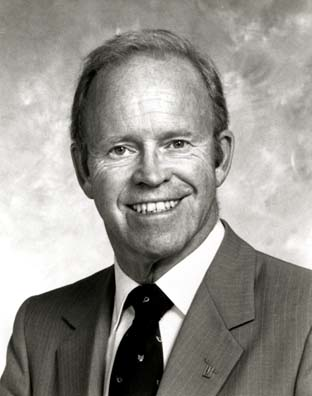
\includegraphics[scale=.3]{img/crosby.png}
    \end{column}
  \end{columns}
\end{frame}

\lecture{Qualidade de Software}{software-quality}

\frame{\title{\insertlecture}\maketitle}

\begin{frame}{\insertlecture}
Não há uma noção clara sobre qualidade de software, pois existem
diferentes pontos de vistas sobre o que vem ser qualidade, e cada
etapa do processo de produção possui características específicas com
critérios diferentes relacionados à qualidade, porém alguns pontos
são listados a seguir:
\pause
\begin{itemize}[<+->]
\item Software sem defeitos.
\item Software adequado ao uso (Juran).
\item Software que atende às especificações (Crosby).
\item Software produzido por uma empresa com certificação.
\item Software que possui confiabilidade, usabilidade, manutenibilidade.
\end{itemize}

\end{frame}

\begin{frame}{Garantia na qualidade de software}

A garantia de qualidade de software (Software Quality Assurance-SQA) é um conjunto de atividades que tem como foco:
\pause
\begin{itemize}[<+->]
\item Minimizar o número de defeitos.
\item Criar mecanismos para controlar o desenvolvimento e a manutenção de forma a preservar prazos e custos.
\item Garantir que o produto possa ser usado no mercado.
\item Melhorar a qualidade de versões futuras dos produtos ou de novos produtos.
\item Os resultados podem ser obtidos através de uma equipe capacitada e uma gestão disciplinada.
\end{itemize}

\end{frame}

\begin{frame}{Qualidade nos processos}

Atividades que podem ser realizadas para melhoria da qualidade.
\pause
\begin{itemize}[<+->]
\item Utilização de padrões nos processos de desenvolvimento que assegura um produto correto, porém, pode não melhorar a qualidade devido a erros técnicos.
\item Inspeção do software/sistema feita por outras pessoas para identificação de erros.
\item Melhoria continua das etapas de cada processo de desenvolvimento.
\item Uso de métricas de da qualidade de software. Porém, as métricas servem como ``bússola'' e devem ser cuidadosamente interpretadas.
\end{itemize}

\end{frame}

\lecture{Normatização}{standard}
\section{\insertlecture}

\begin{frame}{\href{http://www.iso.org/iso/catalogue_detail.htm?csnumber=35733}{Norma ISO/IEC 25010:2011}}%

Substitui a ISO/IEC 9126 e define o modelo de qualidade do processo e
do produto. As atividades definidas para a obtenção da qualidade
durante o desenvolvimento do projeto incluem:
\pause
\begin{itemize}[<+->]
\item Identificação dos requisitos do sistema/software.
\item Validação da compreensão dos requisitos definidos.
\item Identificação dos objetivos do projeto (design) do sistema/software.
\item Identificação dos objetivos do teste dos sistema/software.
\item Identificação dos critérios de controle de qualidade.
\item Identificação dos critérios de aceitação do sistema/software como produto.
\item Estabelecimento de métricas de qualidade que forneçam suporte a estas atividades.
\end{itemize}

\end{frame}

\begin{frame}{Norma \href{https://www.abntcatalogo.com.br/norma.aspx?ID=345041}{ABNT NBR ISO 9001:2015}}

Especifica requisitos para um sistema de gestão de qualidade em
âmbito geral. Possui por objetivos delinear:
\pause
\begin{itemize}
\item Definir atividades para atender os requisitos do cliente, visando
aumentar a satisfação do cliente devido à melhoria de qualidade do
produto atingida pela aplicação destas atividades.
\end{itemize}

\end{frame}

\begin{frame}{Norma \href{https://www.abntcatalogo.com.br/norma.aspx?ID=345041}{ABNT NBR ISO 9001:2015}}
\footnotesize
Uma organização deve seguir alguns passos e atender a alguns
requisitos para serem certificadas:
\pause
\begin{itemize}[<+->]
\item Padronização de todos os processos-chave da organização, processos que afetam o produto e consequentemente o cliente;
\item Monitoramento e medição dos processos de fabricação para assegurar a qualidade do produto/serviço, através de indicadores de performance e desvios;
\item Implementar e manter os registros adequados e necessários para garantir a rastreabilidade do processo;
\item Inspeção de qualidade e meios apropriados de ações corretivas quando necessário; 
\item Revisão sistemática dos processos e do sistema da qualidade para garantir sua eficácia.
\end{itemize}

Um ``produto'', no vocabulário da ISO, pode significar um objeto
físico, ou serviço, ou software. [\href{https://pt.wikipedia.org/wiki/ISO_9000}{Fonte}]

\end{frame}

\begin{frame}{Referência}
\begin{itemize}
\item Mário Lúcio Côrtes; Thelma C. dos Santos Chiossi. ``Modelos de Qualidade de Software''. Editora da UNICAMP, 2001.
\end{itemize}
\end{frame}
